\section{Demonstration}
\begin{frame}{Scenarie}
\begin{columns}
\begin{column}{0.6\textwidth}
Simulering af Hobrovej
\begin{itemize}
\item Dimensioner fra OpenStreetMap
\item Trængsel baseret på GPS målinger og lokalt kendskab
\item Trafiksignaler baseret på 100 sekunders omløbstid
\item Fokus på nordgående retning af Hobrovej
\item SUMO: Mikrosimulator
\item Simulatorens brændstofs- udregninger (HBEFA-baseret)
\item Standardkørsel: Kører efter hastighedsgrænsen når muligt
\end{itemize}
\end{column}

\begin{column}{0.5\textwidth}
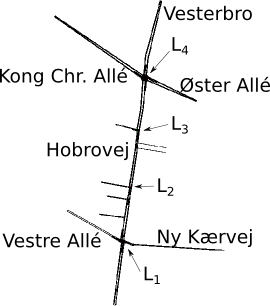
\includegraphics[width=1\textwidth]{../images/HobrovejNy.png}
\end{column}
\end{columns}
\end{frame}

\begin{frame}{Demonstration}
1. Alle kører efter simulatorens standardkørsel
\vspace{4mm}

2. Alle kører med \tech
\begin{itemize}
\item Viser virkningen bedst
\end{itemize}
\end{frame}